\documentclass[a4paper,12pt]{report}
\usepackage[margin=1in]{geometry} % to change the page dimensions
\usepackage{ctex}
\usepackage{xeCJK}
\usepackage{comment}
%\usepackage{times}
\usepackage{setspace}
% \usepackage{lastpage}
\usepackage{fancyhdr}
\usepackage{graphicx}
%\graphicspath{{fig/}}
\usepackage{wrapfig}
\usepackage{subfigure}
\usepackage{array}  
% \usepackage{fontspec,xunicode,xltxtra}
% \renewcommand{\sfdefault}{cmr}
\usepackage{titlesec}
\usepackage{titletoc}
\usepackage[titletoc]{appendix}
%\usepackage[top=30mm,bottom=30mm,left=20mm,right=20mm]{geometry}
%\usepackage{cite}
\usepackage[backend = biber, style = gb7714-2015, defernumbers=true]{biblatex}
%\renewcommand*{\bibfont}{\small}
%\addbibresource{reference.bib}
\setmonofont{Courier New}
\usepackage{listings}
\usepackage{xcolor}
\lstset{tabsize=4, keepspaces=true,
    xleftmargin=2em,xrightmargin=0em, aboveskip=1em,
%    backgroundcolor=\color{FloralWhite},  % 定义背景颜色
    frame=single,                       % 表示不要边框
    extendedchars=false,              % 解决代码跨页时,章节标题,页眉等汉字不显示的问题
    numberstyle=\ttfamily,
    basicstyle=\ttfamily,
    keywordstyle=\color{blue}\bfseries,
    breakindent=10pt,
    identifierstyle=,                 % nothing happens
    commentstyle=\color{red!50!green!50!blue!50},  % 注释的设置
    morecomment=[l][\color{green}]{\#},
    numbers=left,stepnumber=1,numberstyle=\scriptsize,
    showstringspaces=false,
    showspaces=false,
    flexiblecolumns=true,
    breaklines=true, breakautoindent=true,breakindent=4em,
    escapeinside={/*@}{@*/},
}
\usepackage{amsmath}
\usepackage{tikz}
\usetikzlibrary{arrows,shapes,chains}
\usepackage{amsthm}
\newtheorem{theorem}{定理}
\newtheorem{definition}{定义}
\newtheorem{corollary}{推论}
\newtheorem{example}{例}
\usepackage{amsfonts}
%\usepackage{bm}
\usepackage{booktabs} % for much better looking tables
\usepackage{paralist} % very flexible & customisable lists (eg. enumerate/itemize, etc.)
\usepackage{verbatim} % adds environment for commenting out blocks of text & for better verbatim
\usepackage{subfigure} % make it possible to include more than one captioned figure/table in a single float
% These packages are all incorporated in the memoir class to one degree or another...
\usepackage{cases} %equation set
\usepackage{multirow} %use table
\usepackage{algorithm}
\usepackage{algorithmic}
\usepackage{hyperref}
\hypersetup{colorlinks,linkcolor=black,anchorcolor=black,citecolor=black, pdfstartview=FitH,bookmarksnumbered=true,bookmarksopen=true,} % set href in tex & pdf
%\usepackage[framed,numbered,autolinebreaks,useliterate]{mcode} % 插入matlab代码
\XeTeXlinebreaklocale "zh"
\XeTeXlinebreakskip = 0pt plus 1pt minus 0.1pt

%---------------------------------------------------------------------
%	页眉页脚设置
%---------------------------------------------------------------------
\fancypagestyle{plain}{
    \pagestyle{fancy}      %改变章节首页页眉
}

\pagestyle{fancy}
\lhead{\kaishu~何家豪\ 2020211435~}
\rhead{\kaishu~数据结构:约瑟夫问题\ 设计报告}
\cfoot{\thepage}
\titleformat{\chapter}{\centering\zihao{2}\heiti}{第\chinese{chapter}部分}{1em}{}
% \titleformat{\chapter*}{\centering\zihao{-1}\heiti}
\begin{comment}
%---------------------------------------------------------------------
%	章节标题设置
%---------------------------------------------------------------------
\titleformat{\chapter}{\centering\zihao{-1}\heiti}{实验\chinese{chapter}}{1em}{}
\titlespacing{\chapter}{0pt}{*0}{*6}
\end{comment}
%---------------------------------------------------------------------
%	摘要标题设置
%---------------------------------------------------------------------
\renewcommand{\abstractname}{摘要}
\renewcommand{\figurename}{图}
\renewcommand{\tablename}{表}

%---------------------------------------------------------------------
%	参考文献设置
%---------------------------------------------------------------------
%\renewcommand{\bibname}{\zihao{2}{\hspace{\fill}参\hspace{0.5em}考\hspace{0.5em}文\hspace{0.5em}献\hspace{\fill}}}
\renewcommand{\bibname}{参考文献}
\begin{comment}
%---------------------------------------------------------------------
%	引用文献设置为上标
%---------------------------------------------------------------------
\makeatletter
\def\@cite#1#2{\textsuperscript{[{#1\if@tempswa , #2\fi}]}}
\makeatother
\end{comment}
%---------------------------------------------------------------------
%	目录页设置
%---------------------------------------------------------------------
%\renewcommand{\contentsname}{\zihao{-3} 目\quad 录}
\renewcommand{\contentsname}{目录}
\titlecontents{chapter}[0em]{\songti\zihao{-4}}{\thecontentslabel\ }{}
{\hspace{.5em}\titlerule*[4pt]{$\cdot$}\contentspage}
\titlecontents{section}[2em]{\vspace{0.1\baselineskip}\songti\zihao{-4}}{\thecontentslabel\ }{}
{\hspace{.5em}\titlerule*[4pt]{$\cdot$}\contentspage}
\titlecontents{subsection}[4em]{\vspace{0.1\baselineskip}\songti\zihao{-4}}{\thecontentslabel\ }{}
{\hspace{.5em}\titlerule*[4pt]{$\cdot$}\contentspage}

\begin{document}
%---------------------------------------------------------------------
%	封面设置
%---------------------------------------------------------------------
\begin{titlepage}
    \begin{center}
        
    
\includegraphics[width=0.60\textwidth]{bupt_logo.png}\\
    \vspace{10mm}
    \textbf{\zihao{1}{\heiti{北京邮电大学计算机学院}}}\\[0.8cm]
    \textbf{\zihao{1}{\heiti{《数据结构》实验设计报告}}}\\[3cm]
%    \includegraphics[width=0.20\textwidth]{head.jpg}\\%这里是你的照片
    \vspace{\fill}
    
\setlength{\extrarowheight}{3mm}
{\songti\zihao{3}	
\begin{tabular}{rl}
    
    {\makebox[4\ccwd][s]{学\qquad 号:}} & ~\kaishu 2020211435 \\
    {\makebox[4\ccwd][s]{姓\qquad 名:}} & ~\kaishu 何家豪 \\
    {\makebox[4\ccwd][s]{班\qquad 级:}} & ~\kaishu 2020211308\\
%    {\makebox[4\ccwd][s]{专\qquad 业:}} & ~\kaishu 计算机类 \\
    {\makebox[4\ccwd][s]{授课教师:}}  & ~\kaishu 张海旸\\ 
%    {\makebox[4\ccwd][s]{课程助教:}} & ~\kaishu xxx~xxx \\
    {\makebox[4\ccwd][s]{完成日期:}}  & ~\kaishu 2021年10月19日\\ 

\end{tabular}
 }\\[2cm]
%\vspace{\fill}
%\zihao{4}
%使用\LaTeX 撰写于\today
    \end{center}	
\end{titlepage}

%---------------------------------------------------------------------
%  摘要页
%---------------------------------------------------------------------
%\chapter*{摘要}
%    
%这里是摘要。
%
%\textbf{关键词:}总结,理解,思考
%
%\chapter*{Abstract}
%
%This is abstract.
%
%\textbf{Keywords } summary, comprehension, thinking

%---------------------------------------------------------------------
%  目录页
%---------------------------------------------------------------------
\tableofcontents % 生成目录

%---------------------------------------------------------------------
%  绪论
%---------------------------------------------------------------------
\chapter{设计思路}
\setcounter{page}{1}
%\centering
	\tikzstyle{format}=[rectangle,draw,thin,fill=white]  
	%定义语句块的颜色,形状和边
	\tikzstyle{test}=[diamond,aspect=2,draw,thin]  
	%定义条件块的形状,颜色
	\tikzstyle{point}=[coordinate,on grid,] 
	%像素点,用于连接转移线
	\begin{tikzpicture}[node distance=15mm,auto,>=latex',thin,start chain=going below,every join/.style={norm}] 
		%start chain=going below指明了流程图的默认方向,node distance=8mm则指明了默认的node距离。这些可以在定义node的时候更改,比如说 
		%\node[point,right of=n3,node distance=10mm] (p0){};  
%		%这里声明了node p0,它在node n3 的右边,距离是10mm。
		\node[format](start){程序开始};
		\node[format,below of=start] (initList){创建一个空的单链表};
		\node[format,below of=initList](input){读取输入的n的值和其后的n个人,依次插入链表,并输出录入的所有人的信息};
		\node[format,below of=input](link){将单链表的尾结点和头节点首尾相接形成循环链表};
		\node[format, below of=link](inputXMS){读取输入的S,M,X的值};
		\node[format, below of=inputXMS](find){找到ID为S对应的值的人};
		\node[format, below of=find](count){从这个人开始,从1开始报数};
		\node[format, below of=count](kill){数到M,杀死这个人,删除该节点,输出他的个人信息};
		\node[test, below of=kill, node distance=25mm](checkX){检查剩余人数是否为X};
		\node[point, left of=checkX, node distance=75mm](point1){};
		\node[point, left of=count, node distance=75mm](point2){};
		\node[format, below of=checkX, node distance=30mm](printLast){输出剩余X人的信息};
		\node[format, below of=printLast](quit){程序退出};
		
		
		
		\draw[->](start.south) -- (initList);
		\draw[->](initList.south) -- (input);
		\draw[->](input.south) -- (link);
		\draw[->](link.south) -- (inputXMS);
		\draw[->](inputXMS.south) -- (find);
		\draw[->](find.south) -- (count);
		\draw[->](count.south) -- (kill);
		\draw[->](kill.south) -- (checkX);
		\draw[->](checkX) -- node{是}(printLast);
		\draw[-](checkX.west) -- node[above]{否}(point1);
		\draw[-](point1) -- (point2);
		\draw[->](point2) -- node{从删除的下个人开始}(count.west);
		\draw[->](printLast.south) -- (quit);
	\end{tikzpicture}
%---------------------------------------------------------------------
%  极点配置
%---------------------------------------------------------------------
\chapter{代码说明}

\section{常量定义}
\begin{lstlisting}[language=C]
#define NAME_LENGTH 21  // 人名的最大长度
#define MAX_PEOPLE 50  // 最大人数
\end{lstlisting}

\begin{itemize}
    \item NAME\_LENGTH定义了人名的最大长度,考虑到字符串最后的结束符,实际人名最长长度为20。
    \item MAX\_PEOPLE定义了最多的参与人数:50人。
\end{itemize}

\section{结构体定义}
\subsection{人结构体}

\begin{lstlisting}[language=C]
// 定义人结构体
typedef struct Person
{
    int id;        // 编号
    char name[NAME_LENGTH]; // 姓名
    int gender;    // 性别
    int age;       // 年龄
} Person;
\end{lstlisting}
在人结构体中,有人的编号,姓名,性别和年龄。

\subsection{链表结点结构体}
\begin{lstlisting}[language=C]
// 定义链表结点结构体
typedef struct LinkedNode
{
    struct LinkedNode *next; // 指向下一节点
    Person *person;          // 当前人
} Node, *LinkedList;
\end{lstlisting}
在结点的结构体中有指向下一节点的指针域和指向该节点代表的人的结构体指针。这里选择将人的指针作为数据存在结点中,而不是人结构体本身,好处是可以减少在参数传递时的负担。

\section{函数设计及其功能}
	
%\begin{definition}[位姿]
%    位姿是两坐标系间的相互关系,可以等价地用一个位置矢量和一个旋转矩阵来描述:$\left\{ B \right\} = \left\{ {{}_B^AR,{}^A{P_{BORG}}} \right\}$
%\end{definition}
\subsection{initList()}
\begin{lstlisting}[language=C]
// 创建一个带有头节点的空链表
int initList(LinkedList *L)
{
    LinkedList newList = (Node *)malloc(sizeof(Node));  // 为头节点分配空间
    if (!newList)  // 如果空间分配失败
    {
        printf("initList: 创建新链表失败。\n");
        exit(1);
    }
    // 将表头的数据域和指针域置空
    newList->next = NULL;
    newList->person = NULL;
    *L = newList;
    return 0;
}
\end{lstlisting}
该函数的功能是创建一个仅有头节点的空链表。如果在为头结点分配内存时出现错误,将会抛出错误代码1,并退出程序。若创建成功,将会把头结点的指针域和数据域都设置为NULL。头结点将是唯一一个数据域为NULL的结点,这也可以作为后续判断是否为头结点的判断条件。

%\begin{equation}
%    F=ma
%\end{equation}

%---------------------------------------------------------------------
%  分离原则
%---------------------------------------------------------------------
\chapter{运行结果}

\section{运行环境}
\subsection{硬件信息及系统版本}
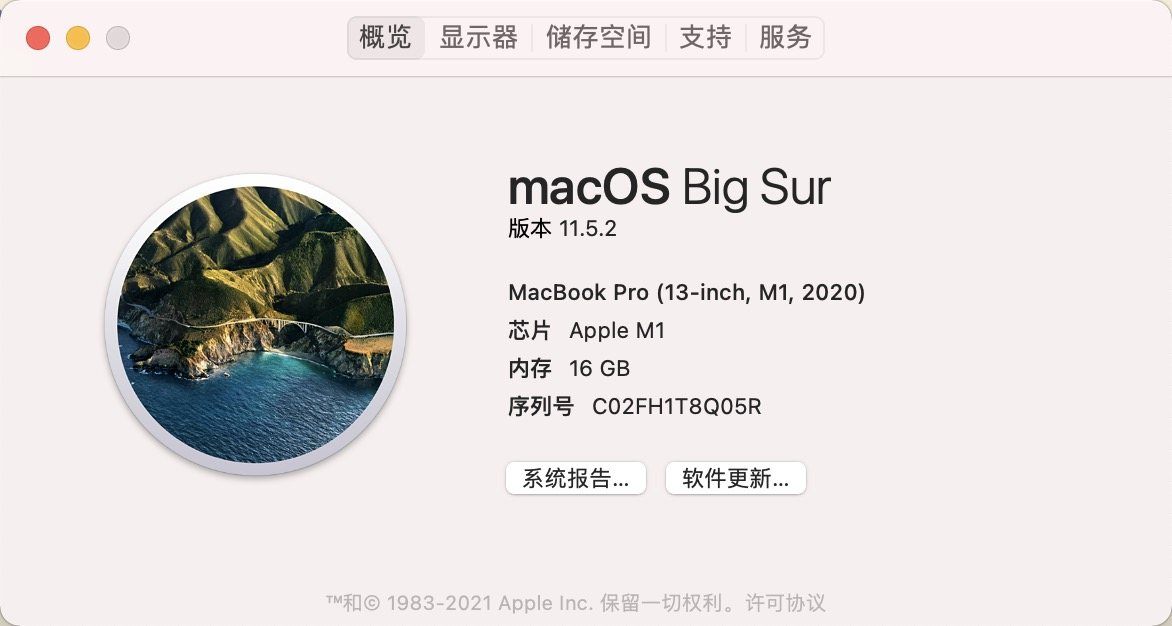
\includegraphics[width=1.00\textwidth]{system_info.png}
\subsection{GCC编译器版本}
\begin{lstlisting}
(base) jasonhe@JasondeMacBook-Pro ~ % gcc --version
Configured with: --prefix=/Applications/Xcode.app/Contents/Developer/usr --with-gxx-include-dir=/Applications/Xcode.app/Contents/Developer/Platforms/MacOSX.platform/Developer/SDKs/MacOSX.sdk/usr/include/c++/4.2.1
Apple clang version 13.0.0 (clang-1300.0.29.3)
Target: arm64-apple-darwin20.6.0
Thread model: posix
InstalledDir: /Applications/Xcode.app/Contents/Developer/Toolchains/XcodeDefault.xctoolchain/usr/bin
\end{lstlisting}
\subsection{编译指令}
本部分的运行结果均是在以下编译指令编译完成后,运行JosephRing可执行文件完成的。
\begin{lstlisting}
(base) jasonhe@JasondeMacBook-Pro ~ % gcc JosephRing.c -o JosephRing
\end{lstlisting}
%\cite{wilson2019learning}采用了sim-to-real learning的架构。

%---------------------------------------------------------------------
%  实验总结
%---------------------------------------------------------------------
%\titleformat{\chapter}{\centering\zihao{-1}\heiti}{}{1em}{}

%---------------------------------------------------------------------
%  参考文献设置
%---------------------------------------------------------------------
%\addcontentsline{toc}{chapter}{参考文献}

%\printbibliography

%\titleformat{\chapter}{\centering\zihao{2}\heiti}{附录~\Alph{chapter}}{1em}{}

%\begin{appendix}
%
%\chapter{第一部分}
%
%\begin{lstlisting}[language=python]
%print('hello world') 
%\end{lstlisting}
%
%\chapter{第二部分}
%
%% Please add the following required packages to your document preamble:
%% \usepackage{booktabs}
%\begin{table}[]
%    \centering
%    \caption{测试结果}
%    \label{tab:my-table}
%    \begin{tabular}{@{}cc@{}}
%    \toprule
%    算法 & 准确率 \\ \midrule
%    I & 0.7684 \\
%    II & 0.7865 \\
%    III & 0.7655 \\ \bottomrule
%    \end{tabular}
%\end{table}
%
%\end{appendix}

\end{document}